% ══════════════════════════════════════════════════════════════════════════
% After Deep CFR — Pluribus, ReBeL, Player of Games, AlphaHoldem
% Companion volume to deep_cfr_tutorial.pdf, same pedagogical style.
% Build:  pdflatex modern_poker_ai_tutorial.tex   (run twice for refs)
% ══════════════════════════════════════════════════════════════════════════
\documentclass[11pt,a4paper]{article}

\usepackage[utf8]{inputenc}
\usepackage[T1]{fontenc}
\usepackage{lmodern}
\usepackage[margin=2.2cm]{geometry}
\usepackage{amsmath,amssymb}
\usepackage[dvipsnames]{xcolor}
\usepackage{tikz}
\usetikzlibrary{arrows.meta,positioning,shapes.geometric,calc,fit,backgrounds}
\usepackage{listings}
\usepackage{tcolorbox}
\usepackage{booktabs}
\usepackage{enumitem}
\usepackage[colorlinks=true,linkcolor=MidnightBlue,urlcolor=MidnightBlue,citecolor=MidnightBlue]{hyperref}

% ─── Palette (same as the Deep CFR tutorial) ────────────────────────────────
\definecolor{accent}{RGB}{25,55,110}
\definecolor{heroG}{RGB}{20,110,60}
\definecolor{villR}{RGB}{160,40,40}
\definecolor{memO}{RGB}{190,110,10}
\definecolor{codebg}{RGB}{246,247,249}
\definecolor{codekw}{RGB}{0,80,160}
\definecolor{codecomment}{RGB}{100,120,100}
\definecolor{codestr}{RGB}{150,60,20}

\lstdefinestyle{py}{
  language=Python,
  basicstyle=\ttfamily\small,
  keywordstyle=\color{codekw}\bfseries,
  commentstyle=\color{codecomment}\itshape,
  stringstyle=\color{codestr},
  backgroundcolor=\color{codebg},
  frame=single, rulecolor=\color{black!25},
  framesep=6pt, xleftmargin=10pt, xrightmargin=4pt,
  showstringspaces=false,
  columns=fullflexible, keepspaces=true,
  breaklines=true
}

\newtcolorbox{intuition}{
  colback=blue!4, colframe=accent, boxrule=0.8pt, arc=2mm,
  title=\textbf{Intuition}, fonttitle=\color{white},
  left=6pt, right=6pt, top=4pt, bottom=4pt}
\newtcolorbox{trap}{
  colback=red!4, colframe=villR, boxrule=0.8pt, arc=2mm,
  title=\textbf{Watch out}, fonttitle=\color{white},
  left=6pt, right=6pt, top=4pt, bottom=4pt}
\newtcolorbox{defbox}{
  colback=black!3, colframe=black!50, boxrule=0.6pt, arc=2mm,
  left=6pt, right=6pt, top=4pt, bottom=4pt}

\setlength{\parskip}{4pt}
\setlength{\parindent}{0pt}

\title{\bfseries After Deep CFR: four modern poker AIs\\[2mm]
\large Pluribus, ReBeL, Player of Games, AlphaHoldem --- a pedagogical tour\\[1mm]
\normalsize Companion volume to \emph{Deep CFR, explained}}
\author{PokerTrainer documentation}
\date{June 2026}

\begin{document}
\maketitle

\begin{abstract}
The companion tutorial \emph{Deep CFR, explained} covered the theory line from
regret matching to Deep CFR. This volume takes the next step and dissects four
landmark systems that followed: \textbf{Pluribus} (superhuman six-player poker
with \emph{no} neural network), \textbf{ReBeL} (reinforcement learning $+$
search on \emph{belief states}), \textbf{Player of Games} (one sound algorithm
for chess, Go \emph{and} poker), and \textbf{AlphaHoldem} (end-to-end deep RL,
no search at all). For each: the one core idea, how it works mechanically
(diagrams $+$ Python pseudo-code), what it achieved, and what it costs.
A final section compares all of them --- including Deep CFR --- on one table and
draws lessons for this project.
\end{abstract}

\tableofcontents
\newpage

% ════════════════════════════════════════════════════════════════════════════
\section{The design space: one map before four deep dives}
% ════════════════════════════════════════════════════════════════════════════

Every poker AI answers two independent questions. \textbf{(1) Where does
game-theoretic reasoning happen?} Offline only (train a strategy, then just
play it), or also \emph{online} (re-solve the current situation at the table)?
\textbf{(2) What stores the strategy?} Tables over abstracted infosets, or
neural networks? The four systems in this volume occupy four distinct corners:

\begin{center}
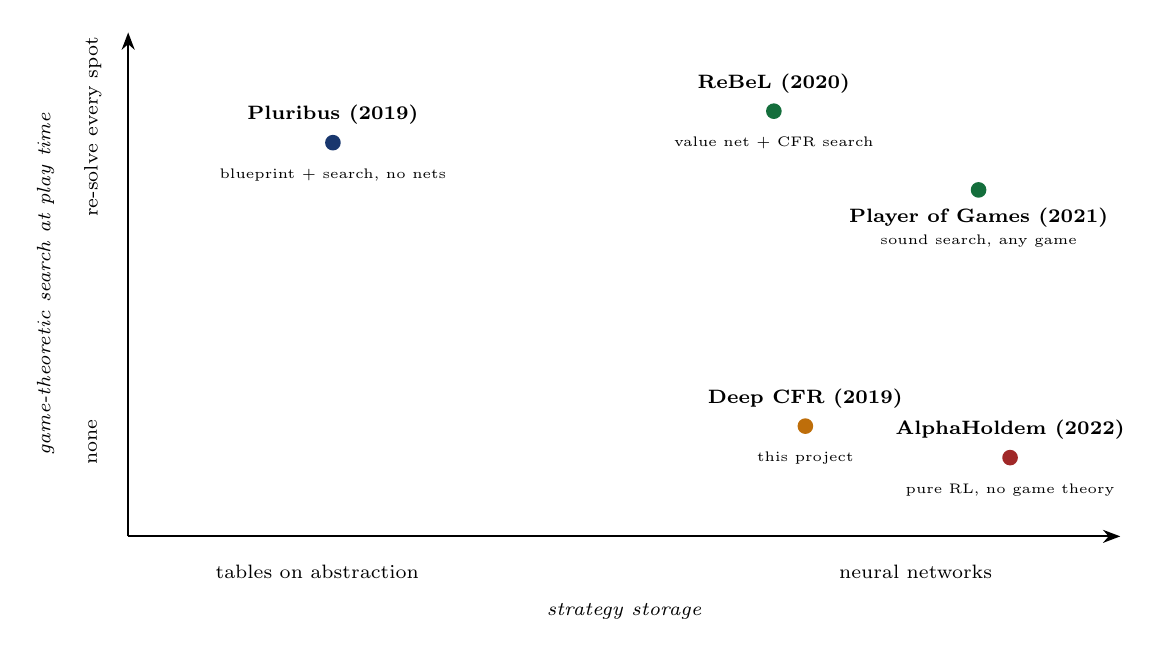
\begin{tikzpicture}[font=\small, >={Stealth[length=2.2mm]}]
  % axes
  \draw[->, thick] (0,0) -- (12.6,0);
  \draw[->, thick] (0,0) -- (0,6.4);
  \node[font=\scriptsize\itshape] at (6.3,-0.95) {strategy storage};
  \node[font=\scriptsize\itshape, rotate=90] at (-1.05,3.2) {game-theoretic search at play time};
  \node[font=\scriptsize] at (2.4,-0.45) {tables on abstraction};
  \node[font=\scriptsize] at (10.0,-0.45) {neural networks};
  \node[font=\scriptsize, rotate=90] at (-0.45,1.2) {none};
  \node[font=\scriptsize, rotate=90] at (-0.45,5.2) {re-solve every spot};

  % systems as dots
  \tikzstyle{sys}=[circle, fill=accent, inner sep=2pt]
  \node[sys, label={[font=\scriptsize\bfseries]above:Pluribus (2019)},
        label={[font=\tiny, yshift=-1mm]below:blueprint + search, no nets}] at (2.6,5.0) {};
  \node[sys, fill=heroG, label={[font=\scriptsize\bfseries]above:ReBeL (2020)},
        label={[font=\tiny, yshift=-1mm]below:value net + CFR search}] at (8.2,5.4) {};
  \node[sys, fill=heroG,
        label={[font=\scriptsize, align=center]below:{\textbf{Player of Games (2021)}\\ \tiny sound search, any game}}] at (10.8,4.4) {};
  \node[sys, fill=memO, label={[font=\scriptsize\bfseries]above:Deep CFR (2019)},
        label={[font=\tiny, yshift=-1mm]below:this project}] at (8.6,1.4) {};
  \node[sys, fill=villR, label={[font=\scriptsize\bfseries]above:AlphaHoldem (2022)},
        label={[font=\tiny, yshift=-1mm]below:pure RL, no game theory}] at (11.2,1.0) {};
\end{tikzpicture}
\end{center}

\begin{intuition}
Read the map as a tug-of-war between two resources: \textbf{offline training
compute} (bottom row pays it all upfront, then plays instantly) and
\textbf{online thinking time} (top row keeps solving at the table, which buys
precision but costs seconds and engineering). The diagonal from Pluribus to
AlphaHoldem is also a diagonal of \emph{decreasing game theory and increasing
deep learning}.
\end{intuition}

% ════════════════════════════════════════════════════════════════════════════
\section{Pluribus: superhuman six-player poker, no neural network}
% ════════════════════════════════════════════════════════════════════════════

\textbf{Paper:} Brown \& Sandholm, \emph{Superhuman AI for multiplayer poker},
Science 2019. \quad
\textbf{One idea:} a coarse offline ``blueprint'' strategy plus cheap
\emph{depth-limited} online re-solving is enough --- even with six players,
even with tables instead of networks.

\subsection{Why six players changes the rules of the game}

Everything in the Deep CFR tutorial relied on the two-player zero-sum
correspondence: regret minimization $\Rightarrow$ Nash, and Nash
$\Rightarrow$ unbeatable. With six players \emph{both} halves break:

\begin{defbox}
In games with $3+$ players, computing a Nash equilibrium is computationally
intractable, and --- worse --- \emph{playing} one is no longer a guarantee:
if the others deviate, your equilibrium share can lose. Pluribus therefore
drops the theoretical target entirely and aims for an \emph{empirical} one:
a strategy that consistently beats elite humans. CFR-style self-play is kept
as a \emph{heuristic} that happens to produce strong, balanced play.
\end{defbox}

\subsection{Stage 1 (offline): the blueprint}

The blueprint is classic pre-deep-learning machinery, exactly what Deep CFR
was designed to replace --- and Pluribus shows it is still viable when paired
with search:

\begin{itemize}[leftmargin=1.4em, itemsep=2pt]
\item \textbf{Information abstraction:} strategically similar hands are
  bucketed (k-means on equity distributions), shrinking $10^{161}$ situations
  to a tractable table.
\item \textbf{Action abstraction:} only a handful of bet sizes exist in the
  abstract game.
\item \textbf{Linear MCCFR} (the same external-sampling traversals as our
  trainer, plus the same linear $t$-weighting) fills the regret tables.
\end{itemize}

The famous headline: the blueprint trained in \textbf{8 days on a 64-core
server}, under 512\,GB RAM, \textbf{no GPU} --- roughly \$150 of cloud compute,
versus millions of dollars of TPU time for Go-class systems.

\subsection{Stage 2 (online): depth-limited re-solving with continuation
strategies}

The blueprint alone is too coarse to beat pros (the abstraction blurs exact
bet sizes and hand distinctions). At the table, Pluribus re-solves the
\emph{current subgame} finely. The problem: a subgame in no-limit poker can
still reach the end of the hand --- far too deep to solve in seconds. The fix
is the paper's key invention:

\begin{center}
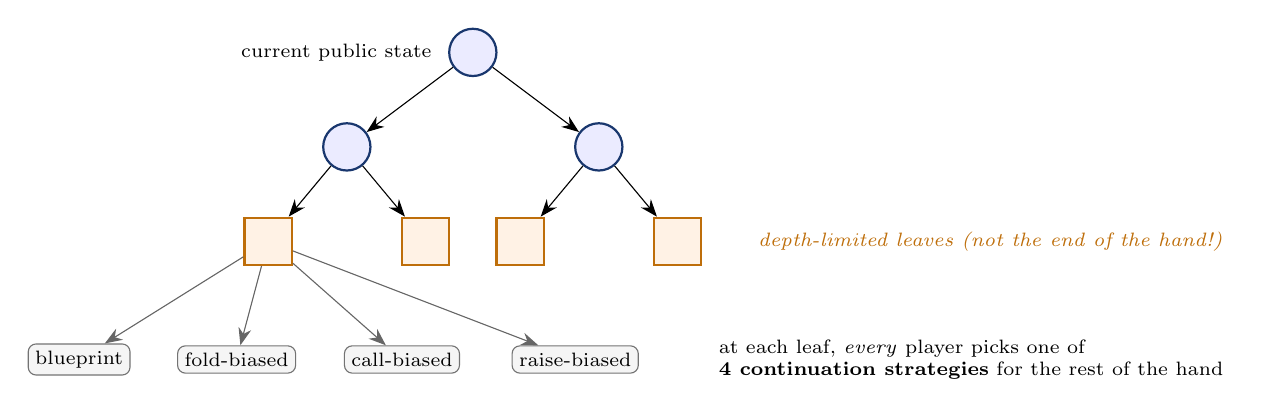
\begin{tikzpicture}[font=\small, >={Stealth[length=2.2mm]},
  nd/.style={circle, draw=accent, fill=blue!8, thick, minimum size=6mm, inner sep=1pt},
  leafnd/.style={rectangle, draw=memO, fill=orange!10, thick, minimum size=6mm, inner sep=2pt},
  cont/.style={rectangle, rounded corners=1mm, draw=black!55, fill=black!4,
               font=\scriptsize, inner sep=2.5pt}]
  % subgame triangle
  \node[nd] (root) at (0,4.2) {};
  \node[font=\scriptsize, anchor=east] at (-0.4,4.2) {current public state};
  \node[nd] (a) at (-1.6,3.0) {};
  \node[nd] (b) at ( 1.6,3.0) {};
  \draw[->] (root) -- (a); \draw[->] (root) -- (b);
  \node[leafnd] (l1) at (-2.6,1.8) {};
  \node[leafnd] (l2) at (-0.6,1.8) {};
  \node[leafnd] (l3) at ( 0.6,1.8) {};
  \node[leafnd] (l4) at ( 2.6,1.8) {};
  \draw[->] (a) -- (l1); \draw[->] (a) -- (l2);
  \draw[->] (b) -- (l3); \draw[->] (b) -- (l4);
  \node[font=\scriptsize\itshape, color=memO, anchor=west] at (3.5,1.8)
    {depth-limited leaves (not the end of the hand!)};

  % continuation fan under one leaf
  \node[cont] (c1) at (-5.0,0.3) {blueprint};
  \node[cont] (c2) at (-3.0,0.3) {fold-biased};
  \node[cont] (c3) at (-0.9,0.3) {call-biased};
  \node[cont] (c4) at ( 1.3,0.3) {raise-biased};
  \draw[->, black!60] (l1) -- (c1);
  \draw[->, black!60] (l1) -- (c2);
  \draw[->, black!60] (l1) -- (c3);
  \draw[->, black!60] (l1) -- (c4);
  \node[font=\scriptsize, align=left, anchor=west] at (3.0,0.3)
    {at each leaf, \emph{every} player picks one of\\
     \textbf{4 continuation strategies} for the rest of the hand};
\end{tikzpicture}
\end{center}

\begin{intuition}
\textbf{Why continuation strategies make shallow leaves honest.} If you
evaluate a leaf with a \emph{single} fixed policy (say, the blueprint), the
search can ``cheat'': it steers play toward leaves where the blueprint plays
badly for the opponent, producing a strategy that only works if the opponent
cooperates. Letting every player \emph{choose among several continuations} at
the leaf is a miniature game: the value of the leaf is what you can get when
the opponent picks their best continuation \emph{against you}. The search can
no longer assume a docile opponent --- at a tiny fraction of the cost of
solving to the end of the hand.
\end{intuition}

\begin{lstlisting}[style=py, caption={Pluribus, schematically. The blueprint is Deep CFR's ancestor (same traversals, tables instead of nets); play time adds depth-limited re-solving.}]
def blueprint(T):                      # OFFLINE, once, ~8 days on CPUs
    for t in range(1, T + 1):
        for p in range(6):             # six players!
            mccfr_traverse(deal(), p, t)   # external sampling, linear weights
    return regret_tables               # indexed by ABSTRACT infosets

def act(public_state, blueprint):      # ONLINE, every decision
    if early_and_on_tree(public_state):
        return sample(blueprint[abstract(public_state)])
    G = subgame(public_state, depth_limit=few_actions)
    for leaf in G.leaves():
        # each player picks 1 of 4 continuations at the leaf -> the leaf
        # itself becomes a small game (no fixed-policy cheating)
        leaf.attach_choices([blueprint, fold_bias, call_bias, raise_bias])
    sigma = linear_cfr(G)              # re-solve the enriched subgame
    return sample(sigma[my_infoset])
\end{lstlisting}

\textbf{Results.} Against elite professionals (including World Series
champions), in both 5 humans $+$ 1 AI and 1 human $+$ 5 copies formats,
Pluribus won decisively. Each decision takes seconds on two CPUs.

\begin{trap}
Pluribus is often summarized as ``deep learning beats poker pros''. It
contains \textbf{no neural network at all}. Its lesson is the opposite of the
hype: \emph{search and good abstractions are devastatingly cost-effective}.
When you read a new-method paper, always ask what a tuned
blueprint-plus-search baseline would have done.
\end{trap}

% ════════════════════════════════════════════════════════════════════════════
\section{ReBeL: reinforcement learning + search on belief states}
% ════════════════════════════════════════════════════════════════════════════

\textbf{Paper:} Brown, Bakhtin, Lerer, Gong, \emph{Combining Deep Reinforcement
Learning and Search for Imperfect-Information Games}, NeurIPS 2020. \quad
\textbf{One idea:} an imperfect-information game becomes a
\emph{perfect-information} game if the ``state'' is taken to be the
\textbf{public belief state} --- then AlphaZero-style self-play $+$ search
applies, with CFR doing the searching.

\subsection{The conversion trick}

\begin{defbox}
\textbf{Public belief state (PBS).} Everything publicly visible (board,
pot, betting history) \emph{plus}, for each player, the probability
distribution over their possible private hands, as computable by an outside
observer who knows both players' strategies. In hold'em each belief is a
vector over the 1326 possible hole-card pairs.
\end{defbox}

Why this works: if both players' policies are common knowledge, then Bayes'
rule updates the beliefs after every public action --- so the PBS evolves
\emph{deterministically given the policies}, like a board position. Hidden
information has been traded for a bigger, continuous state. Values become
well-defined functions of the PBS, so a neural network $V(\mathrm{PBS})$ can
be trained the way AlphaZero trains its value net.

\begin{center}
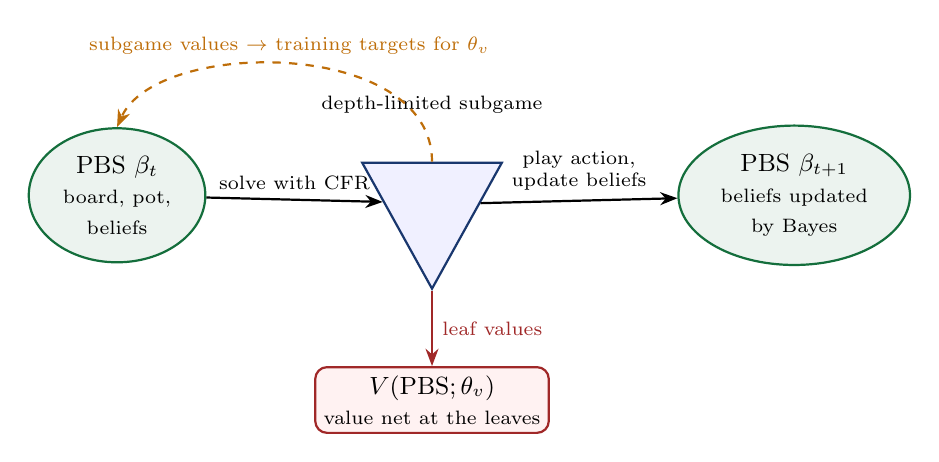
\begin{tikzpicture}[font=\small, >={Stealth[length=2.2mm]},
  pbs/.style={ellipse, draw=heroG, fill=heroG!8, thick, align=center,
              minimum height=10mm, inner sep=3pt},
  sub/.style={isosceles triangle, isosceles triangle apex angle=58, shape border rotate=-90,
              draw=accent, fill=blue!6, thick, minimum height=16mm, inner sep=1pt},
  net/.style={rectangle, rounded corners=1.5mm, draw=villR, fill=red!5, thick,
              align=center, inner sep=3pt}]
  \node[pbs] (b0) at (0,0) {PBS $\beta_t$\\ \scriptsize board, pot,\\ \scriptsize beliefs};
  \node[sub] (g)  at (4.0,-0.1) {};
  \node[font=\scriptsize, align=center, fill=white, inner sep=1pt] at (4.0,1.15)
      {depth-limited subgame};
  \node[net] (v) at (4.0,-2.6) {$V(\mathrm{PBS};\theta_v)$\\ \scriptsize value net at the leaves};
  \node[pbs] (b1) at (8.6,0) {PBS $\beta_{t+1}$\\ \scriptsize beliefs updated\\ \scriptsize by Bayes};

  \draw[->, thick] (b0) -- node[above, font=\scriptsize]{solve with CFR} (g);
  \draw[->, thick, villR] (g.south) -- node[right, font=\scriptsize]{leaf values} (v);
  \draw[->, thick] (g.east) -- node[above, font=\scriptsize, align=center]
      {play action,\\ update beliefs} (b1);
  \draw[->, thick, dashed, memO] (g.north) .. controls (4.0,2.0) and (0.5,2.0) ..
      node[above, font=\scriptsize, color=memO]{subgame values $\to$ training targets for $\theta_v$} (b0.north);
\end{tikzpicture}
\end{center}

\subsection{The self-play loop}

\begin{lstlisting}[style=py, caption={ReBeL's training loop (simplified). The same machinery runs at test time, minus the buffer writes.}]
def rebel_episode(theta_v, theta_pi, buffer):
    beta = initial_pbs()                     # blinds posted, uniform beliefs
    while not beta.is_terminal():
        G = depth_limited_subgame(beta)      # leaves valued by V(.; theta_v)
        policies = run_cfr(G, T_cfr,         # CFR-D: tabular CFR inside G,
                           warm_start=theta_pi)  # net leaf values
        # KEY SUBTLETY: play the policy of a RANDOM CFR iteration, not the
        # final average. This makes the value targets consistent with the
        # distribution of beliefs the next subgame will actually see.
        sigma = policies[randint(1, T_cfr)]
        buffer.add(beta, value_of_root(G, average(policies)))   # V target
        a = sample(sigma[my_private_infoset])
        beta = bayes_update(beta, sigma, a)  # PUBLIC update of both beliefs
    refit(theta_v, buffer)                   # like AlphaZero's value training
\end{lstlisting}

\begin{intuition}
\textbf{Where Deep CFR and ReBeL put the neural network.} Deep CFR's nets
\emph{replace the regret tables} inside one global solve. ReBeL's net replaces
\emph{the bottom of the search tree}: CFR itself stays tabular but only ever
sees a small window of the game, and the net summarizes everything below the
window. That is exactly AlphaZero's division of labor, transplanted to
imperfect information --- which is why the paper's title says ``RL $+$
Search''.
\end{intuition}

\textbf{Results.} Superhuman heads-up no-limit hold'em with far less poker
knowledge than DeepStack/Libratus: it beat top HUNL professional Dong Kim by
\textbf{165\,mbb/hand over 7\,500 hands} (Kim was the best-performing human of
the Libratus match). Also solid play in Liar's Dice, showing generality.

\begin{trap}
\textbf{The PBS is the whole trick --- and the whole bill.} The belief vector
needs one probability per private state: 1326 in hold'em is fine; a game with
$10^{10}$ private states is not. And beliefs are only well-defined if the
policy they are computed from is \emph{common knowledge} --- ReBeL effectively
``announces'' its strategy, which is safe at equilibrium but subtle to reason
about away from it. Porting ReBeL to a new game starts with the question:
\emph{can I even write down the belief vector?}
\end{trap}

% ════════════════════════════════════════════════════════════════════════════
\section{Player of Games: one sound algorithm for chess, Go and poker}
% ════════════════════════════════════════════════════════════════════════════

\textbf{Paper:} Schmid et al., \emph{Player of Games}, 2021; published in
Science Advances 2023 under the name \emph{Student of Games}. \quad
\textbf{One idea:} merge AlphaZero's \emph{growing} search tree with CFR's
\emph{sound} handling of hidden information, so the same agent plays both
kinds of games.

\subsection{What ``sound'' buys you}

AlphaZero's MCTS is built for perfect information; applied naively to poker it
converges to exploitable strategies (it has no concept of balancing a range).
ReBeL is sound but poker-shaped. Player of Games (PoG) asks: what is the
\emph{minimal} unification? Its answer has two components:

\begin{itemize}[leftmargin=1.4em, itemsep=2pt]
\item a \textbf{counterfactual value-and-policy network (CVPN)}: given a public
  state plus beliefs (like ReBeL's PBS), it outputs \emph{per-infoset
  counterfactual values} for both players and a policy prior. In a
  perfect-information game the beliefs are trivial and it degrades exactly to
  AlphaZero's value$+$policy net.
\item \textbf{growing-tree CFR (GT-CFR)}: the search keeps a small
  \emph{public} tree and alternates two phases --- \emph{expand} the tree where
  the policy wants to visit (AlphaZero-style), then run \emph{CFR regret
  updates} over the whole current tree with CVPN values at the leaves.
\end{itemize}

\begin{center}
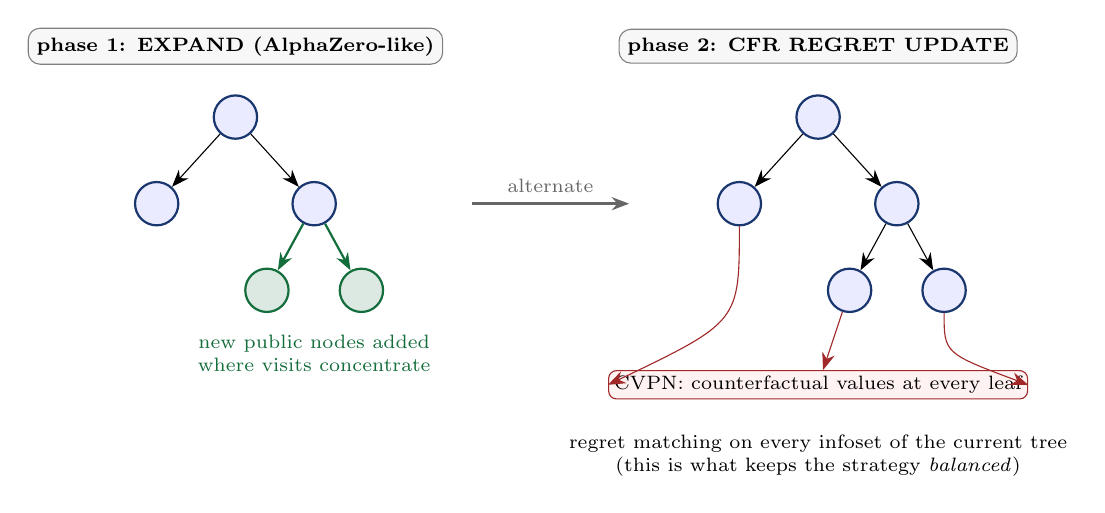
\begin{tikzpicture}[font=\small, >={Stealth[length=2.2mm]},
  nd/.style={circle, draw=accent, fill=blue!8, thick, minimum size=5.5mm, inner sep=1pt},
  newnd/.style={circle, draw=heroG, fill=heroG!15, thick, minimum size=5.5mm, inner sep=1pt},
  phase/.style={rectangle, rounded corners=1.5mm, draw=black!50, fill=black!3,
                font=\scriptsize\bfseries, inner sep=3pt}]
  % phase 1: expansion
  \node[phase] at (1.6,4.9) {phase 1: EXPAND (AlphaZero-like)};
  \node[nd] (r1) at (1.6,4.0) {};
  \node[nd] (a1) at (0.6,2.9) {};
  \node[nd] (b1) at (2.6,2.9) {};
  \newcommand{\dummy}{}
  \node[newnd] (c1) at (2.0,1.8) {};
  \node[newnd] (d1) at (3.2,1.8) {};
  \draw[->] (r1) -- (a1); \draw[->] (r1) -- (b1);
  \draw[->, heroG, thick] (b1) -- (c1); \draw[->, heroG, thick] (b1) -- (d1);
  \node[font=\scriptsize, color=heroG, align=center] at (2.6,1.0)
    {new public nodes added\\ where visits concentrate};

  % phase 2: regret update
  \node[phase] at (9.0,4.9) {phase 2: CFR REGRET UPDATE};
  \node[nd] (r2) at (9.0,4.0) {};
  \node[nd] (a2) at (8.0,2.9) {};
  \node[nd] (b2) at (10.0,2.9) {};
  \node[nd] (c2) at (9.4,1.8) {};
  \node[nd] (d2) at (10.6,1.8) {};
  \draw[->] (r2) -- (a2); \draw[->] (r2) -- (b2);
  \draw[->] (b2) -- (c2); \draw[->] (b2) -- (d2);
  % CVPN at leaves
  \node[rectangle, rounded corners=1mm, draw=villR, fill=red!5, font=\scriptsize,
        inner sep=2pt, align=center] (cvpn) at (9.0,0.6)
        {CVPN: counterfactual values at every leaf};
  \draw[->, villR] (a2) .. controls (8.0,1.4) .. (cvpn.west);
  \draw[->, villR] (c2) -- (cvpn);
  \draw[->, villR] (d2) .. controls (10.6,1.0) .. (cvpn.east);
  \node[font=\scriptsize, align=center] at (9.0,-0.3)
    {regret matching on every infoset of the current tree\\
     (this is what keeps the strategy \emph{balanced})};

  \draw[->, very thick, black!60] (4.6,2.9) -- node[above, font=\scriptsize]{alternate} (6.6,2.9);
\end{tikzpicture}
\end{center}

\begin{lstlisting}[style=py, caption={GT-CFR and sound self-play (schematic).}]
def gt_cfr(beliefs, cvpn, n_rounds):
    tree = PublicTree(root=beliefs)            # starts tiny
    for _ in range(n_rounds):
        for _ in range(E):                     # ── EXPAND ──
            leaf = descend_by_policy_and_visits(tree)
            tree.add_children(leaf, prior=cvpn.policy(leaf))
        for _ in range(R):                     # ── REGRET UPDATE ──
            cfr_iteration(tree, leaf_values=cvpn.values)
    return tree.root_policy(), tree.root_values()

def sound_self_play(cvpn):
    while True:
        traj = play_game(act=lambda b: gt_cfr(b, cvpn, N))
        # every position where the net was queried at a leaf goes into a
        # QUERY BUFFER; a background process re-solves those positions
        # (recursively, with more search) to produce improved value targets
        train(cvpn, value_targets_from(query_buffer), policy_targets_from(traj))
\end{lstlisting}

\begin{intuition}
\textbf{The query buffer is the conceptual heart of the training.} The net is
trained \emph{at exactly the places where the search trusted it} --- each leaf
query becomes a promise to go back later, search deeper from that spot, and
return with a better value to learn from. Compare our project's stage-1 oracle:
the principle ``validate the function where you actually rely on it'' is the
same; PoG just turns it into the training signal itself.
\end{intuition}

\textbf{Results.} One set of weights per game, same algorithm: expert-level
chess and Go (below a specialized AlphaZero at equal compute --- the price of
generality), beats Slumbot (the strongest open heads-up poker bot) and is not
exploited by a local best-response probe, and defeats the state of the art in
Scotland Yard, a hide-and-seek board game with imperfect information.

\begin{trap}
Soundness here is a statement about the \emph{search}, given good values:
more search cannot make play more exploitable. It is not a global optimality
proof, and in perfect-information games generality costs head-to-head strength
versus a specialist. ``One algorithm for everything'' and ``the best algorithm
for each thing'' remain different targets.
\end{trap}

% ════════════════════════════════════════════════════════════════════════════
\section{AlphaHoldem: what if we drop the game theory entirely?}
% ════════════════════════════════════════════════════════════════════════════

\textbf{Paper:} Zhao, Yan, Li, Li, Xing, \emph{AlphaHoldem: High-Performance
Artificial Intelligence for Heads-Up No-Limit Poker via End-to-End
Reinforcement Learning}, AAAI 2022. \quad
\textbf{One idea:} no CFR, no search, no beliefs --- a single network maps the
observation directly to an action, trained with a carefully stabilized PPO
against a pool of past selves.

\subsection{Architecture: two eyes, one brain}

\begin{center}
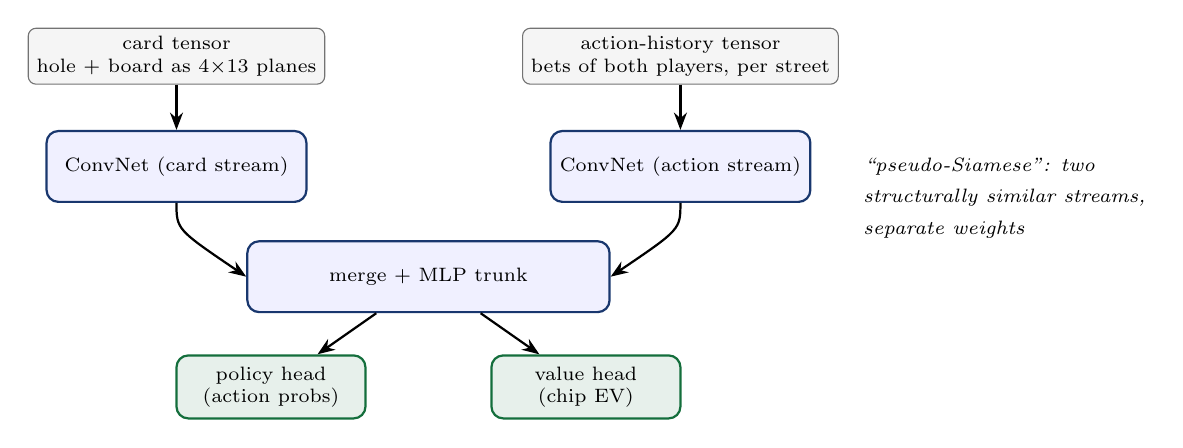
\begin{tikzpicture}[font=\small, >={Stealth[length=2.2mm]},
  inp/.style={rectangle, rounded corners=1mm, draw=black!55, fill=black!4,
              align=center, font=\scriptsize, inner sep=3pt, minimum width=33mm},
  conv/.style={rectangle, rounded corners=1.5mm, draw=accent, fill=blue!6, thick,
               align=center, font=\scriptsize, minimum width=33mm, minimum height=9mm},
  head/.style={rectangle, rounded corners=1.5mm, draw=heroG, fill=heroG!10, thick,
               align=center, font=\scriptsize, minimum width=24mm, minimum height=8mm}]
  \node[inp]  (ci) at (0,3.4)  {card tensor\\ hole + board as $4{\times}13$ planes};
  \node[inp]  (ai) at (6.4,3.4){action-history tensor\\ bets of both players, per street};
  \node[conv] (cc) at (0,2.0)  {ConvNet (card stream)};
  \node[conv] (ac) at (6.4,2.0){ConvNet (action stream)};
  \node[conv, minimum width=46mm] (mlp) at (3.2,0.6) {merge + MLP trunk};
  \node[head] (pol) at (1.2,-0.8) {policy head\\ (action probs)};
  \node[head] (val) at (5.2,-0.8) {value head\\ (chip EV)};
  \draw[->, thick] (ci) -- (cc);
  \draw[->, thick] (ai) -- (ac);
  \draw[->, thick] (cc.south) .. controls (0,1.2) .. (mlp.west);
  \draw[->, thick] (ac.south) .. controls (6.4,1.2) .. (mlp.east);
  \draw[->, thick] (mlp) -- (pol);
  \draw[->, thick] (mlp) -- (val);
  \node[font=\scriptsize\itshape, anchor=west] at (8.6,2.0)
    {``pseudo-Siamese'': two};
  \node[font=\scriptsize\itshape, anchor=west] at (8.6,1.6)
    {structurally similar streams,};
  \node[font=\scriptsize\itshape, anchor=west] at (8.6,1.2)
    {separate weights};
\end{tikzpicture}
\end{center}

Note what is \emph{absent}: no belief vector, no infoset enumeration, no
regret anything. The action history tensor plays the role our token sequence
plays in this project --- it is the only channel through which the network can
infer what the opponent's range looks like.

\subsection{Making PPO survive poker}

Vanilla PPO collapses on poker: rewards span $\pm$200 big blinds with brutal
variance, and importance ratios explode on rare lines. AlphaHoldem's
\textbf{Trinal-Clip PPO} adds two clamps to the standard clipped loss:

\begin{lstlisting}[style=py, caption={Trinal-Clip PPO (the three clips). delta1 caps the policy ratio when the advantage is negative; delta2/delta3 cap the value target at what is physically winnable/losable in the hand.}]
def trinal_clip_losses(ratio, adv, v_pred, v_target, eps, d1, d2, d3):
    # 1+2) standard PPO clip, PLUS an upper cap d1 (> 1+eps) on the ratio
    #      when adv < 0 -- a huge ratio times a negative advantage otherwise
    #      yields an unbounded, variance-exploding policy loss
    r = clip(ratio, 1 - eps, 1 + eps) if adv >= 0 else \
        clip(ratio, 1 - eps, d1)
    policy_loss = -min(ratio * adv, r * adv)
    # 3) value target clipped to the chips actually reachable this hand
    #    (d2 = max losable, d3 = max winnable -- pot/stack dependent)
    value_loss = (v_pred - clip(v_target, -d2, d3)) ** 2
    return policy_loss, value_loss
\end{lstlisting}

\subsection{K-best self-play against strategy cycling}

Naive self-play (always train against the latest self) famously
\emph{cycles} in poker: agent B beats A, C beats B, and C loses to A again ---
rock-paper-scissors in strategy space, no monotone progress. AlphaHoldem
trains each new agent against the \textbf{$K$ best historical versions}
simultaneously, scored by an Elo-like rating; a new agent enters the pool only
if it earns its place. (AlphaStar's league is the same idea at larger scale.)

\begin{lstlisting}[style=py, caption={K-best self-play.}]
pool = [random_init()]
while training:
    learner = clone(best(pool))
    for _ in range(n_steps):
        opponent = sample(pool)                 # mix over the K best
        rollouts = play(learner, opponent)
        update(learner, trinal_clip_ppo(rollouts))
    pool = top_k(pool + [learner], K, by=elo)   # survival of the fittest
\end{lstlisting}

\textbf{Results.} Over 100\,000 evaluation hands, AlphaHoldem beats Slumbot
and a DeepStack re-implementation, after \textbf{3 days of training on one
8-GPU server}, and then decides in \textbf{2.9\,ms} on a single GPU ---
roughly a thousand times faster than search-based systems.

\begin{trap}
\textbf{No theory, no certificate.} Nothing bounds AlphaHoldem's
exploitability; ``beats Slumbot'' does not imply ``cannot be exploited by a
strategy that hunts for its leaks'' --- and follow-up work has indeed found
pure-RL poker agents exploitable. This is the precise trade this corner of the
design-space map makes: spectacular speed and simplicity, no safety net. Our
project's self-play collapses (the 1M-step incoherent policy) were a small
taste of the same phenomenon --- and our stage-1 Nash oracle is exactly the
kind of certificate AlphaHoldem lacks.
\end{trap}

% ════════════════════════════════════════════════════════════════════════════
\section{Side by side, and what this project takes from each}
% ════════════════════════════════════════════════════════════════════════════

\begin{center}
\small
\begin{tabular}{@{}lccccc@{}}
\toprule
 & Deep CFR & Pluribus & ReBeL & PoG/SoG & AlphaHoldem \\
\midrule
year                 & 2019 & 2019 & 2020 & 2021 & 2022 \\
core engine          & CFR  & CFR  & CFR+RL & CFR+MCTS & PPO \\
neural nets          & value+policy & \textbf{none} & value+policy & CVPN & policy+value \\
search at play time  & no   & yes  & yes  & yes  & no \\
belief states needed & no   & no   & yes  & yes  & no \\
abstraction needed   & no   & yes  & no   & no   & no \\
players              & 2    & \textbf{6} & 2 & 2 & 2 \\
theoretical target   & Nash & none (empirical) & Nash & sound search & none \\
training hardware    & GPUs & 64 CPU cores, 8 days & many GPUs & TPUs & 8 GPUs, 3 days \\
decision latency     & ms   & seconds & seconds & seconds & \textbf{2.9 ms} \\
\bottomrule
\end{tabular}
\end{center}

\begin{intuition}
\textbf{Choosing for this project.} PokerTrainer sits in the Deep CFR cell on
purpose: no abstraction to hand-craft (the token transformer reads raw
infosets), no play-time search infrastructure (one network ships in the
Flutter inspector and the C ABI), and a real theoretical target (Nash) that
gives us measurable progress --- which the stage-1 push/fold oracle exploits
directly. The map's other corners tell us what we are giving up: Pluribus-style
re-solving would buy precision at the cost of an online solver; ReBeL/PoG
belief machinery would buy soundness-at-depth at the cost of 1326-dim belief
plumbing; AlphaHoldem's pure RL would buy simplicity at the cost of the very
guarantees we built the oracle to enforce.
\end{intuition}

Concrete techniques worth borrowing here, in increasing order of effort:

\begin{enumerate}[leftmargin=1.6em, itemsep=2pt]
\item \textbf{K-best opponent pools (AlphaHoldem)} --- our evaluation matches
  already revealed self-play drift; rating checkpoints with Elo and evaluating
  new ones against the $K$ best is cheap and directly transplantable.
\item \textbf{Reward/value clipping by reachable chips (AlphaHoldem)} --- the
  same physical bounds ($\pm$ effective stack) we used to reason about regret
  scale apply to any value-learning component we add.
\item \textbf{Continuation-strategy leaf evaluation (Pluribus)} --- if we ever
  add depth limits beyond the current crude bootstrap (flagged in
  \texttt{cfr\_coro.py}), the 4-continuation construction is the principled
  upgrade.
\item \textbf{Query-buffer-style targeted validation (PoG)} --- extend the
  stage-1 oracle idea: log the infosets where the AdvNet's regrets most
  influenced traversals, and audit/validate exactly there.
\end{enumerate}

% ════════════════════════════════════════════════════════════════════════════
\section{Further reading}
% ════════════════════════════════════════════════════════════════════════════

\begin{itemize}[leftmargin=1.4em, itemsep=1pt]
\item Brown, Sandholm (2019). \emph{Superhuman AI for multiplayer poker}
  (Pluribus). Science.
\item Brown, Sandholm (2018). \emph{Depth-Limited Solving for
  Imperfect-Information Games} --- the continuation-strategies construction
  Pluribus builds on.
\item Brown, Bakhtin, Lerer, Gong (2020). \emph{Combining Deep Reinforcement
  Learning and Search for Imperfect-Information Games} (ReBeL). NeurIPS.
\item Schmid et al.\ (2021/2023). \emph{Player of Games} / \emph{Student of
  Games: A unified learning algorithm for both perfect and imperfect
  information games}. Science Advances.
\item Zhao, Yan, Li, Li, Xing (2022). \emph{AlphaHoldem: High-Performance
  Artificial Intelligence for Heads-Up No-Limit Poker via End-to-End
  Reinforcement Learning}. AAAI.
\item Morav\v{c}\'{i}k et al.\ (2017). \emph{DeepStack} --- the origin of
  learned counterfactual values at depth limits, ancestor of both ReBeL and
  PoG.
\item Companion volume: \emph{Deep CFR, explained}
  (\texttt{docs/deep\_cfr\_tutorial/}) --- regret matching, CFR, MCCFR,
  Deep CFR, and this project's curriculum.
\end{itemize}

\end{document}
